\documentclass[tikz,border=10pt]{standalone}
\usetikzlibrary{calc,patterns,angles,quotes,positioning,arrows}

\newcommand{\AxisRotator}[1][rotate=0]{\tikz[x=0.25cm,y=0.60cm,-stealth,#1] \draw (0,0) arc (-150:150:1 and 1);}
\newcommand{\AxisRotatorUnder}[1][rotate=0]{\tikz[x=0.25cm,y=0.60cm,-stealth,#1]
  \draw (0,0) arc (150:-150:1 and 1);}

% \draw (A) -- node[midway] (AMID) {$\AxisRotatorUnder[x=.15cm,y=.36cm,rotate=-45]$} (0,0) -- node[midway] (BMID) {$\AxisRotatorUnder[x=.15cm,y=0.36cm,rotate=45]$} (B);
% \draw[dashed] (-4, 2) node[right] (CA) {$\AxisRotator[x=.15cm,y=.36cm,solid]$} --
%   (4, 2) node [left] (CB) {$\AxisRotator[x=.15cm,y=.36cm,solid]$};


\begin{document}
\begin{figure}[htpb]
 \begin{center}
  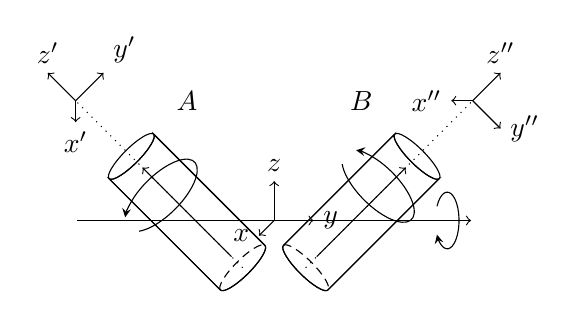
\begin{tikzpicture}[scale=1, transform shape]
    \begin{scope}[shift={(-0.4,0.0)}, rotate=45]
      \node[rotate=-45] at (1.0, 2.0) {$A$};

      \draw (0.4,0) -- (0.4,2.0) arc (360:180:0.4cm and 0.1cm) -- (-0.4,0) arc
      (180:360:0.4cm and 0.1cm);
      \draw (-0.4,2.0) -- (-0.4,0) arc (180:360:0.4cm and 0.1cm) -- (0.4,2.0) ++
      (-0.4,0) circle (0.4cm and 0.1cm);
      \draw[densely dashed] (-0.4,0) arc (180:0:0.4cm and 0.1cm);
      \draw[->] (0,0.2) -- (0,1.8) node[below]{$\AxisRotator[x=0.60cm,y=0.25cm]$};
      \draw[dotted] (0,0)--(0,3);
      \draw[->](0.0,3.0,0.0) -- (0.5, 3.0,0.0) node[above right,rotate=-45]{$y'$};
      \draw[->](0.0,3.0,0.) -- (0.0, 3.5,0.0) node[above,rotate=-45]{$z'$};
      \draw[->](0.0,3.0,0.0) -- (0.0, 3.0,0.5) node[below,rotate=-45]{$x'$};
    \end{scope}
    \begin{scope}[shift={(0.4,0.0)}, rotate=-45]
      \node[rotate=45] at (-1.0, 2.0) {$B$};

      \draw (0.4,0) -- (0.4,2.0) arc (360:180:0.4cm and 0.1cm) -- (-0.4,0) arc
      (180:360:0.4cm and 0.1cm);
      \draw (-0.4,2.0) -- (-0.4,0) arc (180:360:0.4cm and 0.1cm) -- (0.4,2.0) ++
      (-0.4,0) circle (0.4cm and 0.1cm);
      \draw[densely dashed] (-0.4,0) arc (180:0:0.4cm and 0.1cm);
      \draw[->] (0,0.2) -- (0,1.8) node[below]{$\AxisRotator[x=0.60cm,y=0.25cm]$};
      \draw[dotted] (0,0)--(0,3);
      \draw[->](0.0,3.0,0.0) -- (0.5, 3.0,0.0) node[right,rotate=45]{$y''$};
      \draw[->](0.0,3.0,0.) -- (0.0, 3.5,0.0) node[above,rotate=45]{$z''$};
      \draw[->](0.0,3.0,0.0) -- (0.0, 3.0,0.5) node[left,rotate=45]{$x''$};
    \end{scope}
    \draw[->] (-2.5,0.6)--(2.5,0.6) node[left]
    {$\AxisRotatorUnder[x=0.15cm,y=0.36cm]$};
    \draw[->](0.0,0.6,0.0) -- (0.5, 0.6,0.0) node[right]{$y$};
    \draw[->](0.0,0.6,0.) -- (0.0, 1.1,0.0) node[above]{$z$};
    \draw[->](0.0,0.6,0.0) -- (0.0, 0.6,0.5) node[left]{$x$};
  \end{tikzpicture}
   \end{center}
\end{figure}
\end{document}
